%!TEX program = xelatex

%----------------------------------------------------------------------------------------
%	PACKAGES AND OTHER DOCUMENT CONFIGURATIONS
%----------------------------------------------------------------------------------------

\documentclass[
	12pt, % Default font size, select one of 10pt, 11pt or 12pt
	fleqn, % Left align equations
	a4paper, % Paper size, use either 'a4paper' for A4 size or 'letterpaper' for US letter size
	%oneside, % Uncomment for oneside mode, this doesn't start new chapters and parts on odd pages (adding an empty page if required), this mode is more suitable if the book is to be read on a screen instead of printed
]{myLegrandOrangeBook}

% Book information for PDF metadata, remove/comment this block if not required 
\hypersetup{
	pdftitle={Title}, % Title field
	pdfauthor={Author}, % Author field
	pdfsubject={Subject}, % Subject field
	pdfkeywords={Keyword1, Keyword2, ...}, % Keywords
	pdfcreator={LaTeX}, % Content creator field
}

% 所用包
\usepackage[dvipsnames]{xcolor}
\usepackage{fancyhdr}
\usepackage{extramarks}
\usepackage{amsmath}
\usepackage{amsthm}
\usepackage{amsfonts}
\usepackage{tikz}
\usepackage[plain]{algorithm}
\usepackage{algpseudocode}
\usepackage{ctex}
\usepackage{indentfirst}
\usepackage{wrapfig}
\usetikzlibrary{automata,positioning,shapes.geometric,arrows.meta,patterns,calc}

% 我的newcommand
\newcommand{\degree}{^{\circ}}
\newcommand{\arrow}{-{Stealth[length=4mm,width=2mm]}}
\newcommand{\rmd}{\mathrm{d}}
\newcommand{\deriv}[2]{\frac{\rmd #1}{\rmd #2}}
\renewcommand{\parallel}{\mathrel{/\mskip-2.5mu/}}

\addbibresource{reference.bib} % Bibliography file

\definecolor{ocre}{RGB}{243, 102, 25} % Define the color used for highlighting throughout the book

\chapterimage{miku3.png} % Chapter heading image
\chapterspaceabove{6.5cm} % Default whitespace from the top of the page to the chapter title on chapter pages
\chapterspacebelow{6.75cm} % Default amount of vertical whitespace from the top margin to the start of the text on chapter pages

%----------------------------------------------------------------------------------------

\begin{document}

%----------------------------------------------------------------------------------------
%	TITLE PAGE
%----------------------------------------------------------------------------------------

\titlepage % Output the title page
	{\includegraphics[width=\paperwidth]{miku0.jpg}} % Code to output the background image, which should be the same dimensions as the paper to fill the page entirely; leave empty for no background image
	{ % Title(s) and author(s)
		\centering\sffamily % Font styling
		{\Huge\bfseries University Physics\par} % Book title
		\vspace{16pt} % Vertical whitespace
		{\LARGE Notes\par} % Subtitle
		\vspace{24pt} % Vertical whitespace
		{\huge\bfseries Lai Wei\par} % Author name
	}

%----------------------------------------------------------------------------------------
%	TABLE OF CONTENTS
%----------------------------------------------------------------------------------------

\pagestyle{empty} % Disable headers and footers for the following pages

\tableofcontents % Output the table of contents

\pagestyle{fancy} % Enable default headers and footers again

\cleardoublepage % Start the following content on a new page

%----------------------------------------------------------------------------------------
%	PART
%----------------------------------------------------------------------------------------

\part{大学物理A1}

%----------------------------------------------------------------------------------------
%	SECTIONING EXAMPLES CHAPTER
%----------------------------------------------------------------------------------------

\chapterimage{miku2.jpg} % Chapter heading image
\chapterspaceabove{6.75cm} % Whitespace from the top of the page to the chapter title on chapter pages
\chapterspacebelow{7.25cm} % Amount of vertical whitespace from the top margin to the start of the text on chapter pages

%------------------------------------------------

\chapter{质点运动学}

\section{质点力学}

\subsection{参考系、质点}

\subsubsection*{参考系}

    为描述物体运动而选的标准物。

\subsubsection*{参考系}

    物体能否视为质点视具体情况而定。

\subsubsection*{坐标系}

    定量描述物体运动。坐标系的原点一般固定在参照系上。

    \begin{enumerate}
        \item 直角坐标系\(\left(x,y,z\right)\)
        \item 球坐标系\(\left(r,\theta,\varphi\right)\):二维极坐标
        \item 柱坐标系\(\left(\rho,\varphi,z\right)\)
        \item 自然坐标系\(s\)
    \end{enumerate}

\subsection{位置矢量、运动方程、路程、位移}

\subsubsection*{位置矢量}

    \begin{wrapfigure}{r}{4cm}
        \centering
        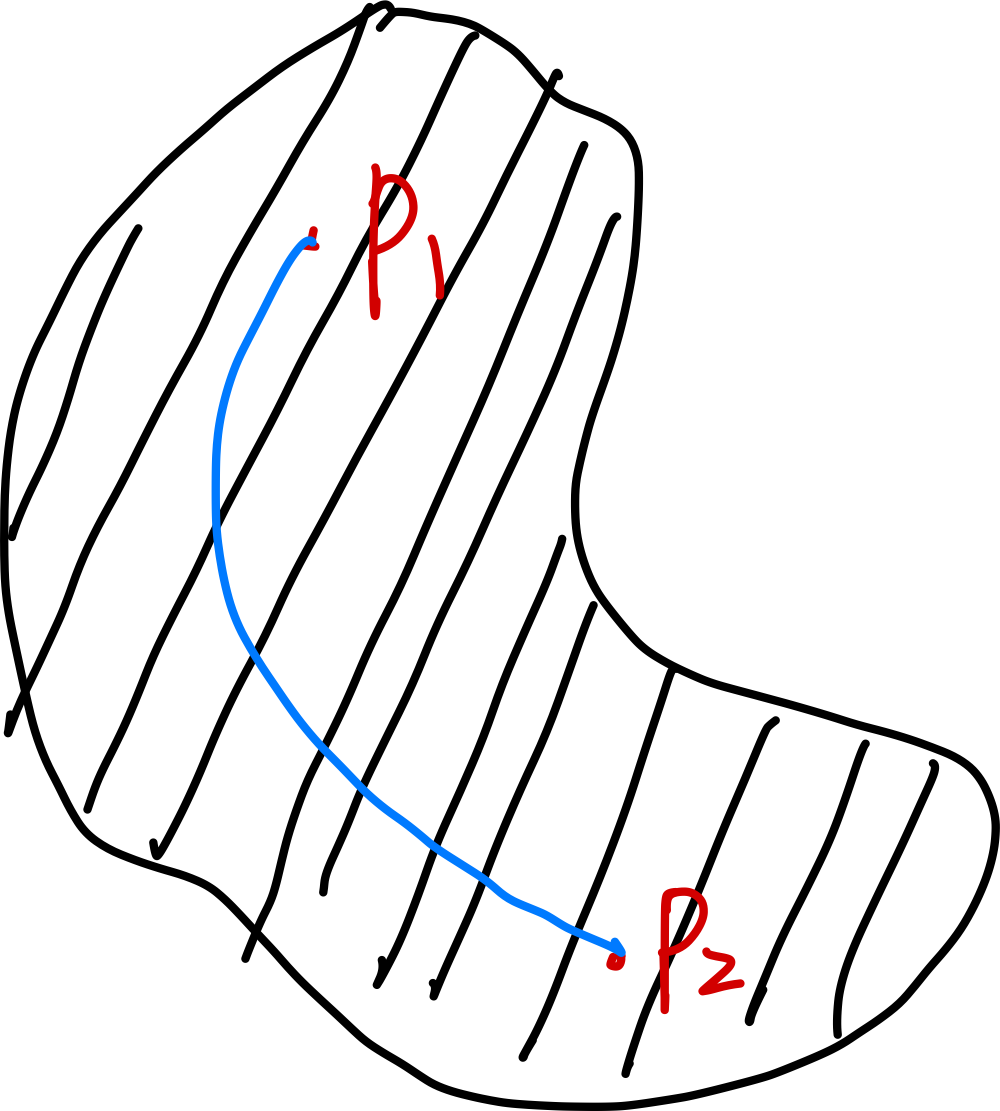
\includegraphics[scale=0.08]{"Chapter 01 images/pic1.png"}
        % \caption{}
        \label{pic1}
    \end{wrapfigure}

    \begin{align*}
        \overrightarrow{r} &= x\overrightarrow{i} + y\overrightarrow{j} + z\overrightarrow{k} \\
        r &= \left|\overrightarrow{r}\right| = \sqrt{x^2 + y^2 + z^2}
    \end{align*}

    \(\overrightarrow{r}\)的方向可以用一组方向角,即\(\overrightarrow{r}\)与\(x\)轴、
    \(y\)轴、\(z\)轴之间的夹角\(\left(\alpha, \beta, \gamma\right)\)来表示。
    \(\cos \alpha = \frac{x}{r}\)、\(\cos \beta = \frac{y}{r}\)、\(\cos \gamma = \frac{z}{r}\),
    有\(\cos \alpha ^2 + \cos \beta ^2 + \cos \gamma ^2 = 1\)。

\subsubsection*{运动方程(直角坐标系下)}
    
    \begin{wrapfigure}{r}{4cm}
        \centering
        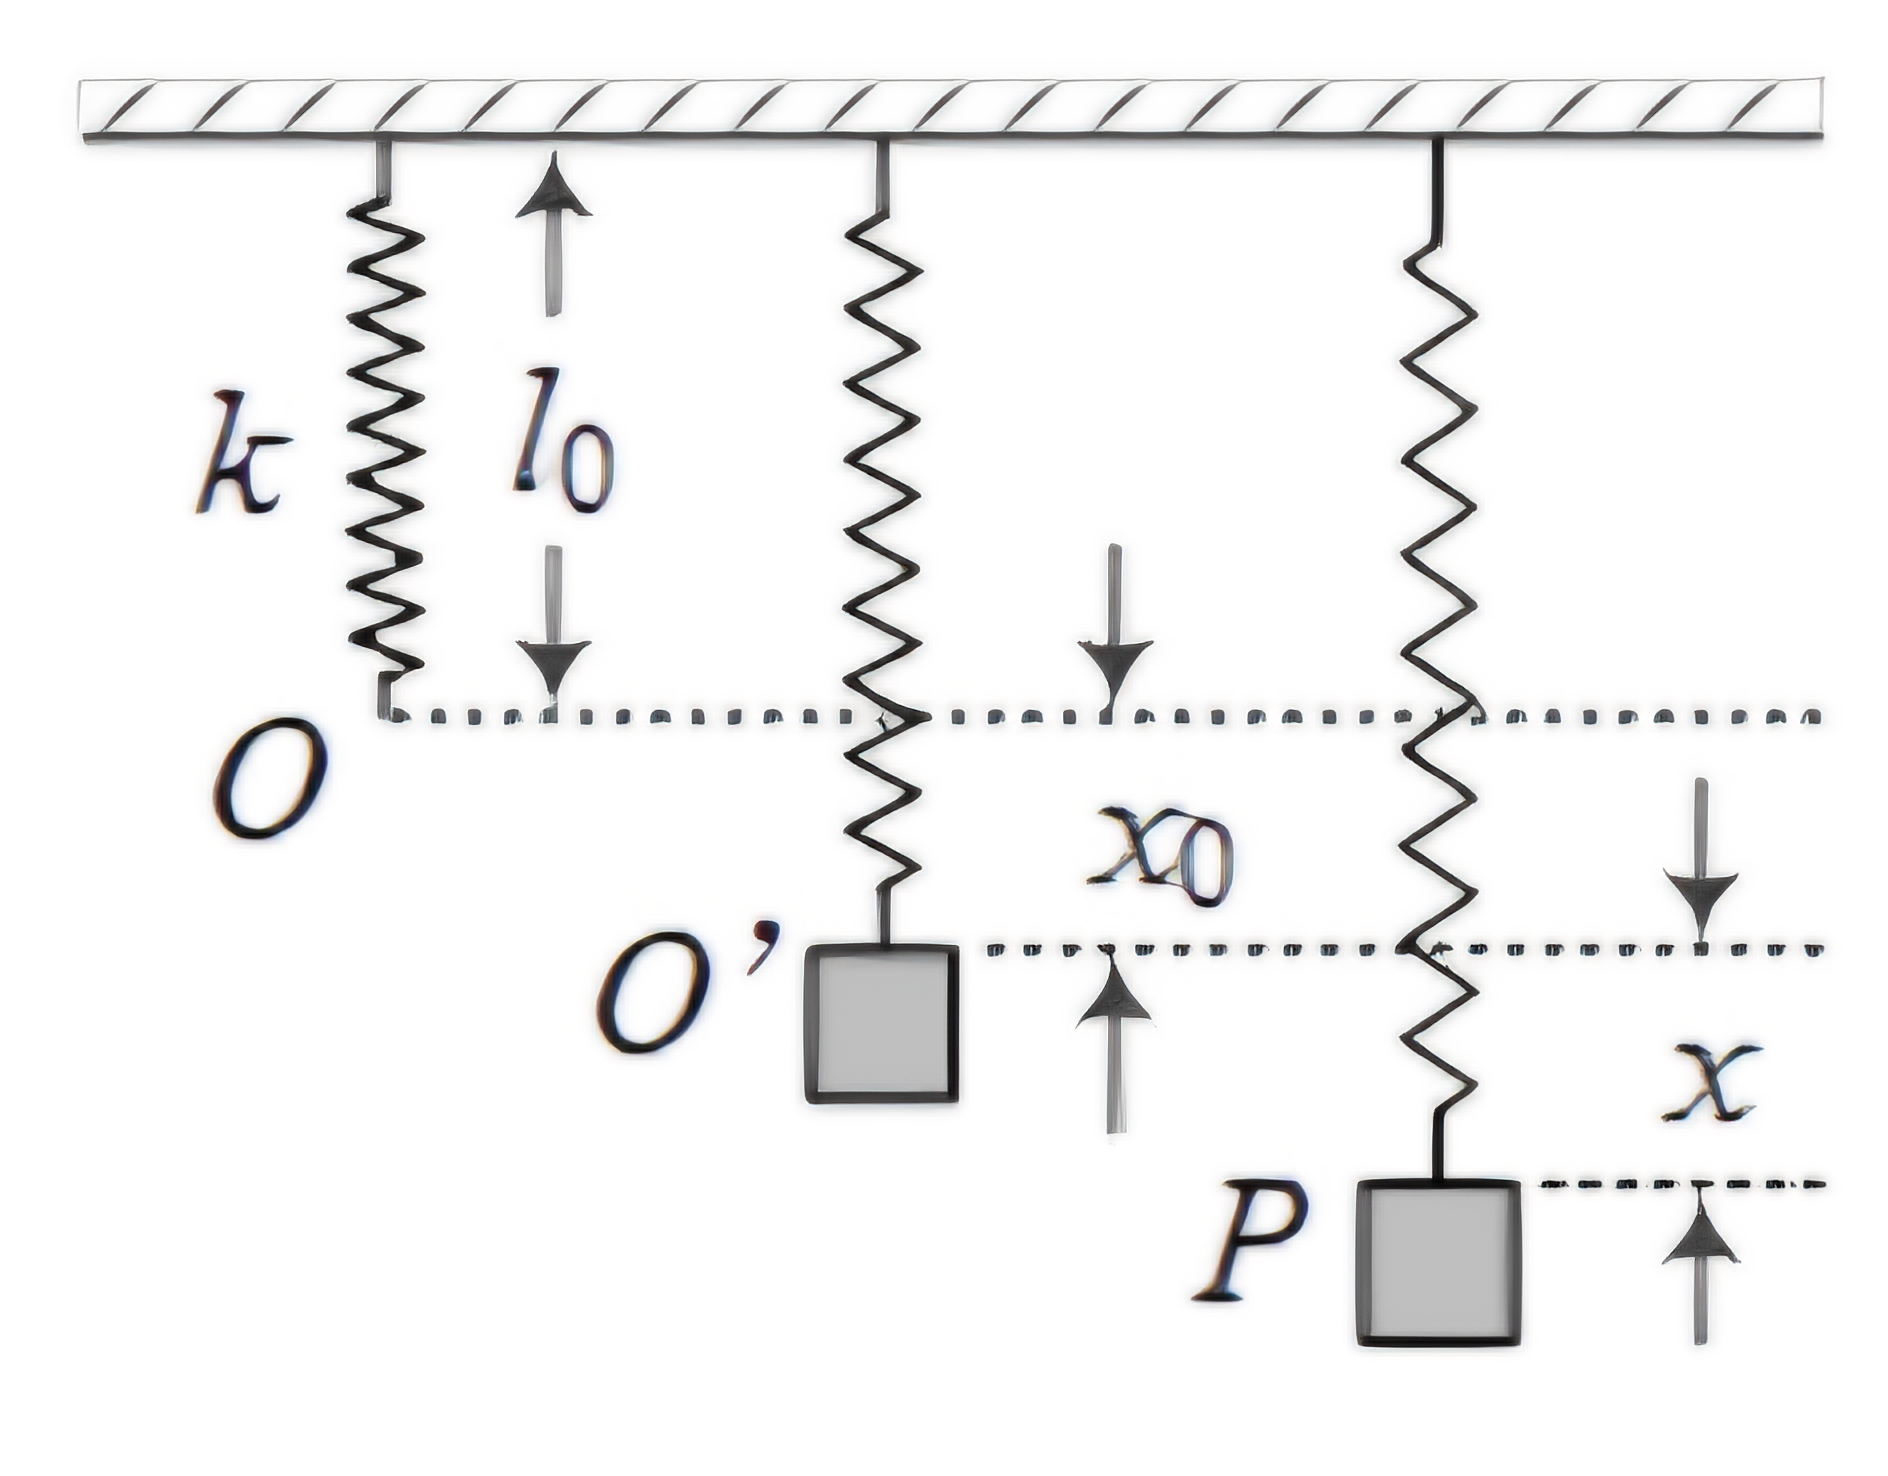
\includegraphics[scale=0.08]{"Chapter 01 images/pic2.png"}
        % \caption{}
        \label{pic2}
    \end{wrapfigure}

    \[
        \overrightarrow{r}\left(t\right) = 
        x\overrightarrow{i}\left(t\right) + y\overrightarrow{j}\left(t\right)
        + z\overrightarrow{k}\left(t\right)
    \]

    分量式

    \[
    \begin{cases}
    x = x\left(t\right), \\
    y = y\left(t\right), \\ 
    z = z\left(t\right).
    \end{cases}
    \]

    从上式中消去参数得质点的{\heiti 轨迹方程}。

\subsection{位移、路程}

\subsubsection*{位移\(\Delta \overrightarrow{r}\)(位置矢量的改变量)}


    \begin{wrapfigure}{r}{4cm}
        \centering
        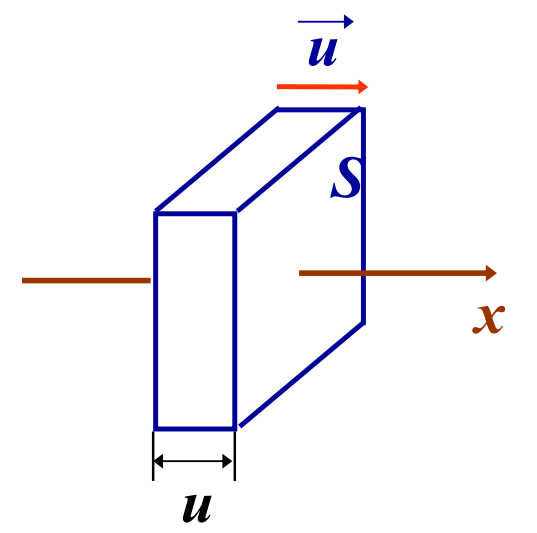
\includegraphics[scale=0.08]{"Chapter 01 images/pic3.png"}
        % \caption{}
        \label{pic3}
    \end{wrapfigure}

    \begin{align*}
        \overrightarrow{r_{A}} &=
        x_{A}\overrightarrow{i} + y_{A}\overrightarrow{j} + z_{A}\overrightarrow{k}
        ,\; \left(t_{A}\text{时}\right) \\
        \overrightarrow{r_{B}} &=
        x_{B}\overrightarrow{i} + y_{B}\overrightarrow{j} + z_{B}\overrightarrow{k}
        ,\; \left(t_{B}\text{时}\right)
    \end{align*}

    于是其位移

    \[\Delta \overrightarrow{r} = \overrightarrow{r_{B}} - \overrightarrow{r_{A}}
    = \left(x_{B} - x_{A}\right)\overrightarrow{i} + \left(y_{B} - y_{A}\right)\overrightarrow{j}
    + \left(z_{B} - z_{A}\right)\overrightarrow{k}
    \]
    
    方向由\(A\)指向\(B\)。

\subsubsection*{路程\(\Delta s\)实际轨迹}

    \begin{wrapfigure}{r}{4cm}
        \centering
        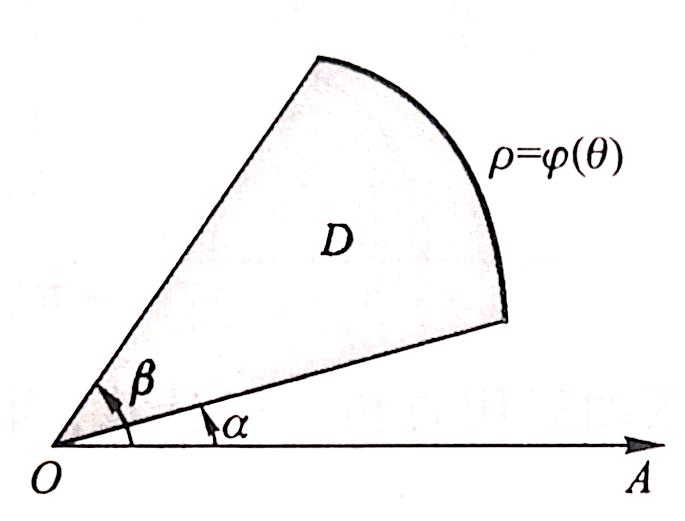
\includegraphics[scale=0.05]{"Chapter 01 images/pic4.png"}
        % \caption{}
        \label{pic4}
    \end{wrapfigure}

    从\(P_{1}\)到\(P_{2}\),路程记为\(\Delta s = \hat{P_{1}P_{2}}\)。

    位移与路程的区别:

    \begin{enumerate}
        \item 位移是适量,路程是标量;
        \item 两点之间位移是唯一的,路程不是唯一的;
        \item 一般情况下,\(\left|\Delta \overrightarrow{r}\right| \neq \Delta s\)
            \\
            在方向不变的圆周运动中,\(\left|\Delta \overrightarrow{r}\right| = \Delta s\)
            当\(\Delta t \rightarrow 0\)时,\(\left| \rmd \overrightarrow{r}\right| = \rmd s\)
            (元位移\(\rmd \overrightarrow{r} = \rmd x \overrightarrow{i} +
            \rmd y \overrightarrow{j} + \rmd z \overrightarrow{k}\))。
    \end{enumerate}

\subsection{速度}

\subsubsection*{平均速度}

    \begin{wrapfigure}{r}{4cm}
        \centering
        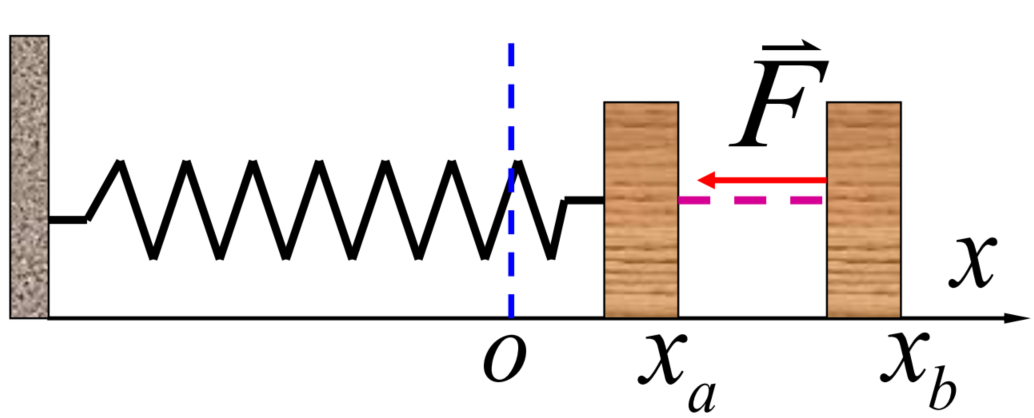
\includegraphics[scale=0.08]{"Chapter 01 images/pic5.png"}
        % \caption{}
        \label{pic5}
    \end{wrapfigure}

    在\(\Delta t\)内,质点位移(二维)为

    \begin{align*}
        \Delta \overrightarrow{r} &= \overrightarrow{r} \left(t + \Delta t\right) -
        \overrightarrow{r} \left(t\right)
        \\
        &= \Delta x \overrightarrow{i} + \Delta y \overrightarrow{j}
    \end{align*}

    \textbf{定义}
    \[
    \overrightarrow{v} = \frac{\Delta \overrightarrow{r}}{\Delta t} =
    \frac{\Delta x}{\Delta t} \overrightarrow{i} + \frac{\Delta y}{\Delta y} \overrightarrow{j}
    \]

\subsubsection*{瞬时速度}

    当\(\Delta t \rightarrow 0\)时,

    \begin{align*}
        \overrightarrow{v} = \lim_{\Delta t \rightarrow 0}\frac{\Delta \overrightarrow{r}}{\Delta t}
        &= \frac{\rmd \overrightarrow{r}}{\rmd t}
        \\
        &= \frac{\rmd x}{\rmd t} \overrightarrow{i} + \frac{\rmd y}{\rmd t} \overrightarrow{j}
        + \frac{\rmd z}{\rmd t} \overrightarrow{k}
        \\
        & = v_{x} \overrightarrow{i} + v_{y} \overrightarrow{j} + v_{z} \overrightarrow{k}
    \end{align*}

    即有,

    \[
    v_{x} = \frac{\rmd x}{\rmd t},\; v_{y} = \frac{\rmd y}{\rmd t},\; v_{z} = \frac{\rmd z}{\rmd t}
    \]

    所以

    \[
    \left|\overrightarrow{v} \right| = \sqrt{\left(\frac{\rmd y}{\rmd t}\right)^2 +
    \left(\frac{\rmd y}{\rmd t}\right)^2 + \left(\frac{\rmd z}{\rmd t}\right)^2}
    \]

    方向角

    \[
        \cos \alpha = \frac{v_x}{v},\; \cos \beta = \frac{v_y}{v}, \;\cos \gamma = \frac{v_z}{v}
    \]

    习惯上,二维情况下,用\(\tan \theta = \frac{v_y}{v_x}\)表示方向。

    同理,速率\(v = \frac{\rmd s}{\rmd t}\),而因为\(t \rightarrow 0\)时,
    有\(\left|\overrightarrow{r}\right| = s\),则

    \[
    v = \left|\overrightarrow{v}\right| =
    \left|\frac{\rmd \overrightarrow{r}}{\rmd t}\right|
    = \frac{\left|\rmd \overrightarrow{r}\right|}{\rmd t}
    = \frac{\rmd s}{\rmd t}
    \]

    即有,速度的大小等于速率。

\subsubsection*{速度在自然坐标系下的表示}

    \[
    \overrightarrow{v} = \frac{\rmd s}{\rmd t}\overrightarrow{e_{t}}
    = v \overrightarrow{e_{t}}
    \]

    其中,\(\overrightarrow{e_{t}} = 1\),表示方向,\(v\)表示速度大小。

\subsection{加速度}

    反应速度大小和方向随时间变化快慢。

\subsubsection*{平均加速度}

    \begin{wrapfigure}{r}{4cm}
        \centering
        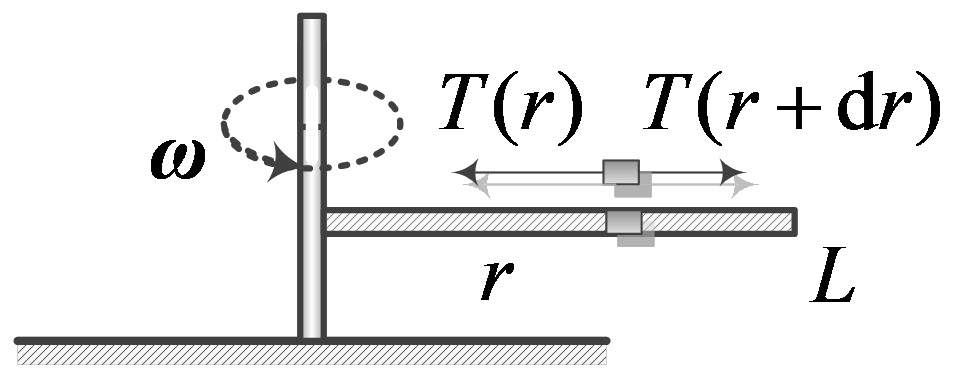
\includegraphics[scale=0.08]{"Chapter 01 images/pic6.png"}
        % \caption{}
        \label{pic6}
    \end{wrapfigure}


    \[
    \overline{\overrightarrow{a}} = \frac{\Delta \overrightarrow{v}}{\Delta t}
    \]

    \(\overrightarrow{a}\)与\(\Delta \overrightarrow{v}\)的方向相同。

\subsubsection*{瞬时加速度}

    特点:

    \begin{enumerate}
        \item {\color{Thistle}"矢量性"}
        \item {\color{Thistle}"瞬时性"}
        \item {\color{Thistle}"相对性"}(相对于某一参考系)
    \end{enumerate}

    \begin{align*}
    \overrightarrow{a} &= \lim_{\Delta t \rightarrow 0} \frac{\Delta \overrightarrow{v}}{\Delta t}
    = \frac{\rmd \overrightarrow{v}}{\rmd t} =
    \frac{\rmd^2 \overrightarrow{r}}{\rmd t^2}
    \\
    &= \frac{\rmd v_{x}}{\rmd t} \overrightarrow{i} +
    \frac{\rmd v_{y}}{\rmd t} \overrightarrow{j} +
    \frac{\rmd v_{z}}{\rmd t} \overrightarrow{k}
    \\
    &= a_{x}\overrightarrow{i} + a_{y}\overrightarrow{j}
    + a_{z}\overrightarrow{k}
    \end{align*}

    方向角\(\alpha\)、\(\beta\)和\(\gamma\)满足

    \[
        \cos \alpha = \frac{a_x}{a},\; \cos \beta = \frac{a_y}{a}, \;\cos \gamma = \frac{a_z}{a}
    \]

    习惯上,二维时方向表示为\(\tan \theta = \frac{a_y}{a_x}\)。
    
    \begin{wrapfigure}{r}{4cm}
        \centering
        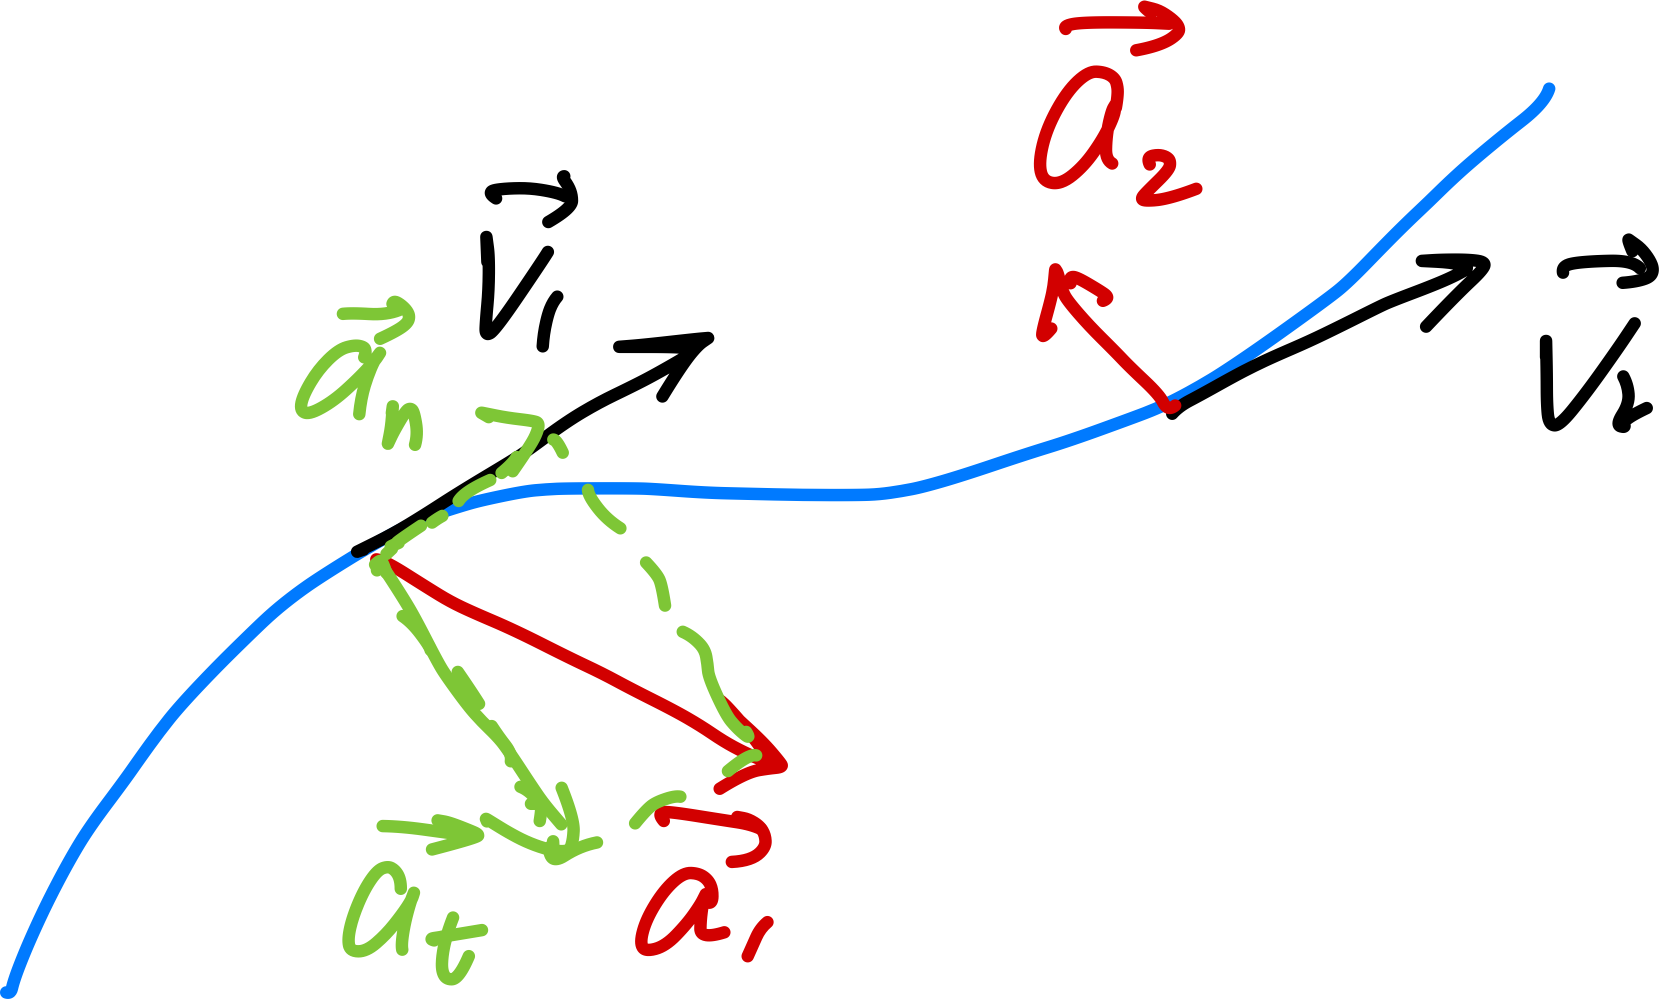
\includegraphics[scale=0.05]{"Chapter 01 images/pic7.png"}
        % \caption{}
        \label{pic7}
    \end{wrapfigure}

    加速度的方向:

    \begin{itemize}
        \item 直线运动:\(\overrightarrow{a} \parallel \overrightarrow{v}\)。
        \item 曲线运动:指向轨迹凹测。
            自然坐标系下,\(\overrightarrow{a} = \overrightarrow{a_{n}} + \overrightarrow{a_{t}}\)。
    \end{itemize}

    在变速曲线运动中,加速度的方向总是指向轨迹凹的一侧。与\(\overrightarrow{v}\)呈锐角时,运动变快;
    与\(\overrightarrow{v}\)呈钝角时,运动变快。(因为\(\Delta \overrightarrow{v}\)必定指向曲线凹的一侧。)

\subsection{例题}


    在离水面高为\(h\)的岸上,有人用绳拉船靠岸,如图所示。设人以匀速率\(v_{0}\)收绳,试求:
    当船距岸边\(x_{0}\)时,船的速度和加速度的大小各是多少?

    \[
        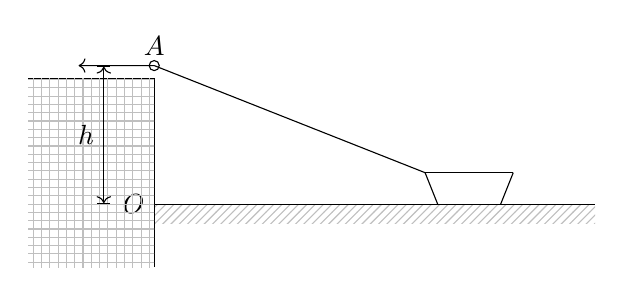
\begin{tikzpicture}[scale=0.8]
        \coordinate[label=left:$O$] (O) at (0,0);
        \coordinate[label=above:$A$] (A) at (0,2.2);
        \fill[pattern=north east lines, pattern color=gray!50] (0,0) rectangle (7,-0.3);
        \draw (0,-1) -- (0,2);
        \draw (O) -- (7,0);
        \draw (0,2) -- (-2,2);
        \fill[pattern=grid, pattern color=gray!50] (0,-1) rectangle (-2,2);
        \draw (A) circle (0.08);
        % 小船
        \draw (4.5,0) -- (5.5,0);
        \draw (4.5,0) -- (4.3,0.5);
        \draw (5.5,0) -- (5.7,0.5);
        \draw (4.3,0.5) -- (5.7,0.5);
        % 绳子
        \draw (A) -- (4.3,0.5);
        \draw[->] (A) -- (-1.2,2.2);
        % 尺寸标注
        \draw[|<->|] (-0.8,0) -- (-0.8,2.2) node[midway, left] {$h$};
        \end{tikzpicture}
    \]
    \\

    \textbf{Solution}
    \\

    \textbf{Part One}

    建立如图所示的坐标系。

    \[
        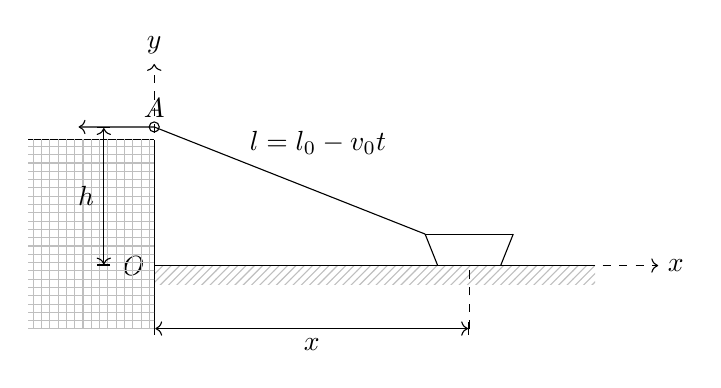
\begin{tikzpicture}[scale=0.8]
        \coordinate[label=left:$O$] (O) at (0,0);
        \coordinate[label=above:$A$] (A) at (0,2.2);
        \fill[pattern=north east lines, pattern color=gray!50] (0,0) rectangle (7,-0.3);
        \draw (0,-1) -- (0,2);
        \draw (O) -- (7,0);
        \draw (0,2) -- (-2,2);
        \fill[pattern=grid, pattern color=gray!50] (0,-1) rectangle (-2,2);
        \draw (A) circle (0.08);
        % 小船
        \draw (4.5,0) -- (5.5,0);
        \draw (4.5,0) -- (4.3,0.5);
        \draw (5.5,0) -- (5.7,0.5);
        \draw (4.3,0.5) -- (5.7,0.5);
        % 绳子
        \draw (A) -- (4.3,0.5);
        \draw[->] (A) -- (-1.2,2.2);
        \coordinate[label={above:$ l = l_{0} - v_{0}t $}] (rope) at (2.6,1.6);
        % 尺寸标注
        \draw[|<->|] (-0.8,0) -- (-0.8,2.2) node[midway, left] {$h$};
        \draw[|<->|] (0,-1) -- (5,-1) node[midway, below] {$x$};
        \draw[dashed] (5,-1) -- (5,0);
        % 坐标系
        \coordinate[label=right:$x$] (x) at (8,0);
        \coordinate[label=above:$y$] (y) at (0,3.2);
        \draw[->,dashed] (O) -- (x);
        \draw[->,dashed] (O) -- (y);
        \end{tikzpicture}
    \]

    设初始时刻,船与岸上\(A\)点之间的绳长为\(l_{0}\)。在任意时刻船离岸边的距离为\(x\),
    绳长为\(l_{0}\)。船在运动过程中,\(l\)和\(x\)均是时间\(t\)的函数。

    由题意,\(l = l_{0} - v_{0}t\),所以

    \[
    v_{0} = - \deriv{l}{t}
    \]

    又由几何关系

    \[
    l^{2} = x^{2} + h^{2}
    \]

    对上式两边同时对\(t\)求导,可得

    \[
    2 l \deriv{l}{t} = 2x \deriv{x}{t}
    \]

    则船的运动速度为

    \[
    v = \deriv{x}{t} = \frac{l}{x} \deriv{l}{t} = -\frac{l}{x} v_{0}
    \]
    \\

    \textbf{Part Two}

    再将速度对时间\(t\)求导,即可得到船的加速度为

    \[
    a = \deriv{v}{t} = - \frac{v_{0}}{x^{2}} \left(x \deriv{l}{t} - l \deriv{x}{t}\right)
    = -\frac{v_{0}^{2} h^{2}}{x^{3}}
    \]
    \\

    \textbf{Part Three}

    令\(x=x_{0}\),得船在离岸边为\(x_{0}\)时的速度和加速度分别为

    \[
    v = \frac{\sqrt{x_{0}^{2} + h^2}}{x_{0}} v_{0},\;
    a = -\frac{v_{0}^{2} h^{2}}{x_{0}^{3}}
    \]



%----------------------------------------------------------------------------------------
%	PRESENTING INFORMATION/RESULTS EXAMPLES CHAPTER
%----------------------------------------------------------------------------------------

% \chapterimage{orange3.jpg} % Chapter heading image
% \chapterspaceabove{6.25cm} % Whitespace from the top of the page to the chapter title on chapter pages
% \chapterspacebelow{7.5cm} % Amount of vertical whitespace from the top margin to the start of the text on chapter pages

%----------------------------------------------------------------------------------------

\end{document}
